\paragraph{Performance of the $\alpha$-strategy.}
\begin{figure*}[!ht]
	\centering
	\subfloat[Percentage of arrivals completed by the deadlines.]{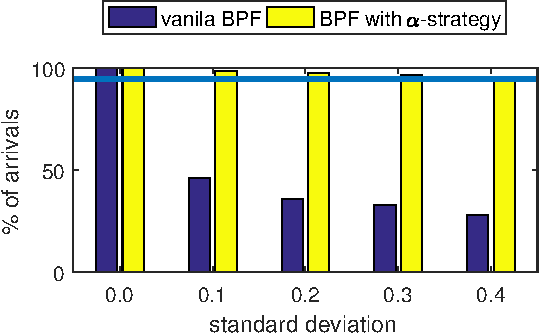
\includegraphics[width=0.3\linewidth]{fig/probabilistic_result} \label{fig:probabilistic_result}}
	\hspace{0.2cm}
	\subfloat[Requested demand normalized by that under the vanilla \name. ]{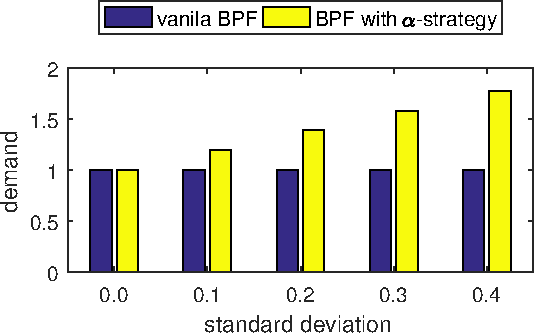
\includegraphics[width=0.3\linewidth]{fig/probabilistic_provision} \label{fig:probabilistic_provision}}	
	\hspace{0.2cm}
	\subfloat[Resource consumption of LQ.]{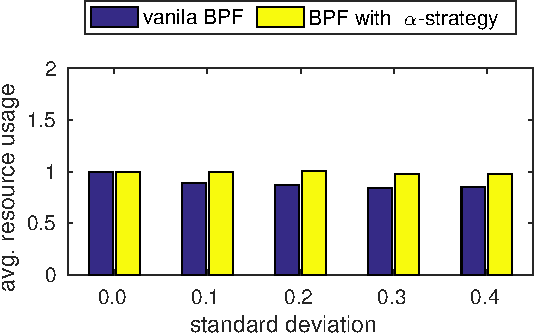
\includegraphics[width=0.3\linewidth]{fig/prob_avg_res} \label{fig:prob_avg_res}}
	\caption{[Simulation] The proposed $\alpha$-strategy under $\alpha$=95\% is robust against the uncertainties.}
	\label{fig:probabilistic}
	\vspace{-0.3cm}
\end{figure*}

Figure~\ref{fig:probabilistic} depicts the requested demand, performance, and resource usage under the vanilla \name and the one with the $\alpha$-strategy when arrivals have different sizes. In particular, as the variance increases, the vanilla \name can no longer complete $\alpha$ arrivals before the deadline. Actually, even with 10\% standard deviation, the percentage drops below 50\%. On the other side, \name with $\alpha$-strategy always satisfy the $\alpha$ requirement. Even though the reported demand increases, the average resource usage does not change much, e.g., \batchq still receives the same long-term share.



%\todo{Change the 95 percentile to BPF with $\alpha$-strategy. Change mean to vanilla BPF. Make the 95\% line thicker and remove it from the legend. Change reported demand of (a)'s y-axis to demand. Change (b)'s y-axis to \% of arrivals. Switch the order of (a) and (b)}